\documentclass[11pt]{article}
\usepackage{amsmath, amssymb, amsthm}
\usepackage[retainorgcmds]{IEEEtrantools}

\usepackage[pdftex]{graphicx}
\usepackage{tikz}
\usepackage{circuitikz}
\usetikzlibrary{intersections}

\usepackage{fancyhdr}

%Format stuff
\pagestyle{fancy}
\headheight 35pt

%Header info
\chead{\Large \textbf{Interference and Diffraction}}
\lhead{}
\rhead{}

\begin{document}
\section{Two Beam Interference}
	Imagine two identical beams (modeled by traveling waves) pointed at the same point:
	\begin{center}
	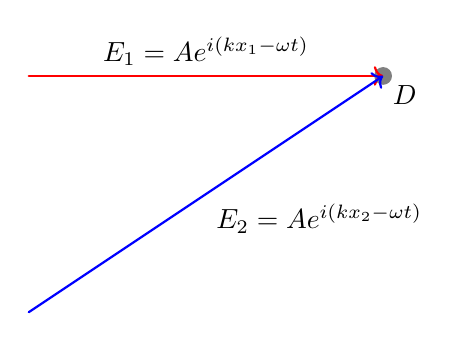
\begin{tikzpicture}
		[scale=1.5,line cap=round,
		%Styles
		axes/.style=,
		important line/.style={very thick},
		information text/.style={rounded corners,fill=red!10,inner sep=1ex},
		dot/.style={circle,inner sep=1pt,fill,label={#1},name=#1}			
		]
		
		%Colors
		\colorlet{anglecolor}{green!50!black}	%angle arcs/lines
		
		%The graphic
		\filldraw[color=gray] (3, 0) node[below right,black] {$D$} circle (2pt);
		\draw[->,thick,red] (0, 0) -- node[above,black] {$E_1 = Ae^{i(kx_1-\omega t)}$} (3, 0);
		\draw[->,thick,blue] (0, -2) -- node[below right,black] {$E_2 = Ae^{i(kx_2 - \omega t)}$} (3, 0);
	\end{tikzpicture}
	\end{center}
	These two beams will exhibit interference at $D$. The combined wave at that point is then
	\begin{IEEEeqnarray}{rCl}
		E_p = E_1 + E_2 & = & 2Ae^{i(k\bar{x} - \omega t)}\cos\left( \frac{k\delta}{2} \right)\\
		\delta & = & x_2 - x_1\\
		\bar{x} & = & \frac{x_1 + x_2}{2}
	\end{IEEEeqnarray}
	The cosine term is called the \textbf{amplitude factor} and the exponential is called the \textbf{wave factor}. 
	
	Usually for analysis, we discard the wave factor because it is oscillating too fast to observe. If we only want the amplitude factor, or the \textbf{intensity} of the resultant wave. The intensity is proportional to the amplitude squared, as follows:
	\begin{equation}
		I \propto E_p E_p^* = 4A^2\cos^2\frac{k\delta}{2}
	\end{equation}
	For a single beam, this result would be $A^2$, but the superimposed wave has an amplitude factor that has to be factored in. Note that for interfering beams of equal intensity, the intensity maximum is 4 times what it would be for one beam.
	
	In general, to observe interference we need the beams to have the same polarization and coherent waves. Polarization is usually achieved by using the same source to create the two beams, but real light waves are not perfect cosine functions. This means that we need to choose a source with as long of \textbf{coherence time}, the amount of time the light wave remains predictable, and \textbf{coherence length}, the distance that a light wave remains predictable. For example, He-Ne lasers have coherence lengths of 20cm-10m, whereas white light has a coherence length of about one wavelength.
	
\section{Michelson Interferometer}
	The Michelson interferometer splits a single beam of light into two paths, bouncing the beams back and recombining them by using two mirrors and a half-silvered mirror.

	\begin{center}
	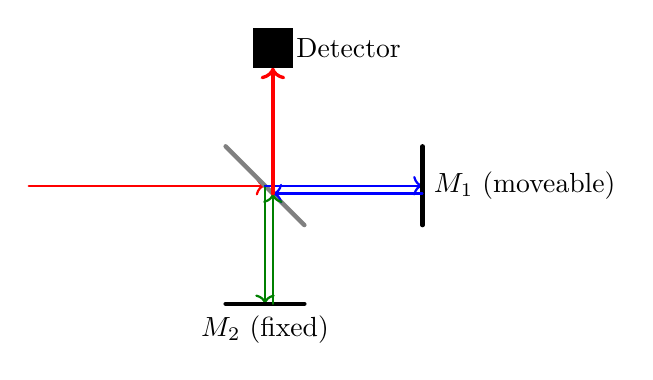
\begin{tikzpicture}
		[scale=1,line cap=round,
		%Styles
		axes/.style=,
		important line/.style={very thick},
		information text/.style={rounded corners,fill=red!10,inner sep=1ex},
		dot/.style={circle,inner sep=1pt,fill,label={#1},name=#1}			
		]
		
		%Colors
		\colorlet{anglecolor}{green!50!black}	%angle arcs/lines
		
		%The graphic
		\draw[red,->,thick] (0, 0) -- (3, 0);
		\draw[gray,ultra thick] (2.5, .5) -- (3.5, -.5);
		\draw[anglecolor,->,thick] (3, 0) -- (3, -1.5);
		\draw[blue,->,thick] (3, 0) -- (5, 0);
		
		\draw[black,ultra thick] (2.5, -1.5) -- node[below] {$M_2$ (fixed)} (3.5, -1.5);
		\draw[black,ultra thick] (5, .5) -- node[right] {$M_1$ (moveable)} (5, -.5);
		
		\draw[blue,->,thick] (5, -.1) -- (3.1, -.1);
		\draw[anglecolor,->,thick] (3.1, -1.5) -- (3.1, -.1);
		
		\draw[red,->,very thick] (3.1, -.1) -- (3.1, 1.5);
		\filldraw[black] (2.85, 2) rectangle node[right=5pt,black] {Detector} (3.35, 1.5);
	\end{tikzpicture}
	\end{center}
	
	There are two source of phase shift in this device. The first source is the difference in the distance the two halves of the split beam have to travel, and the second is the interval reflection off the glass along $M_1$.
	\begin{IEEEeqnarray}{rCl}
		\Delta x & = & 2(x_1 - x_2) = \delta\\
		\Delta \phi_\delta & = & 2k(x_1 - x_2)\\
		\Delta \phi_i & = & \pi
	\end{IEEEeqnarray}
	The total phase difference is then $\Delta \phi = 2k(x_2 - x_1) + \pi$.
	
	Changing $x_2$ changes the phase shifts between destructive and constructive interference. For totally constructive interference, the waves are in phase (i.e. $\Delta \phi = m \cdot 2\pi$), and for totally destructive interference, the waves are exactly opposite in phase (i.e. $\Delta \phi = m\pi$).
	
	For a given \textbf{fringe order} $m \in \{0, 1, 2, \ldots\}$ then, the Michelson interferometer will exhibit totally constructive interference when
	\begin{equation}
		\frac{2(x_2 - x_1)}{\lambda} = m \pm \frac{1}{2}
	\end{equation}
	and totally destructive interference when
	\begin{equation}
		\frac{2(x_2 - x_1)}{\lambda} = m
	\end{equation}
	Because $m$ is the number of rings (fringes) in the resulting wave at the detector, we can use it to calculate the wavelength of the source wave:
	\begin{equation}
		\Delta m = \frac{2(x_2 - x_1)}{\lambda}
	\end{equation}
	
\section{Single-Slit Diffraction}
	When a beam of light encounters a single slit, it diffracts into spherical wave rays. The pattern of these wave rays can be captured on a screen set some distance away if a lens is placed to move the diffraction pattern from a convergence point at infinity.
	
	\begin{center}
	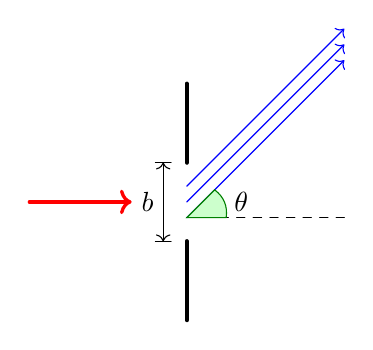
\begin{tikzpicture}
		[scale=1,line cap=round,
		%Styles
		axes/.style=,
		important line/.style={very thick},
		information text/.style={rounded corners,fill=red!10,inner sep=1ex},
		dot/.style={circle,inner sep=1pt,fill,label={#1},name=#1}			
		]
		
		%Colors
		\colorlet{anglecolor}{green!50!black}	%angle arcs/lines
		
		%The graphic
		\draw[black,ultra thick] (0, 1.5) -- (0, .5);
		\draw[black,ultra thick] (0, -1.5) -- (0, -.5);
		
		\draw[red,very thick,->] (-2, 0) -- (-.7, 0);
		\draw[<->] (-.3, .5) -- node[left] {$b$} (-.3, -.5);
		\draw (-.4, .5) -- (-.2, .5);
		\draw (-.4, -.5) -- (-.2, -.5);
		
		\draw[blue,->] (0, .2) -- (2, 2.2);
		\draw[blue,->] (0, 0) -- (2, 2);
		\draw[blue,->] (0, -.2) -- (2, 1.8);
		
		\draw[dashed] (0, -.2) -- (2, -.2);
		
		\coordinate (A) at (2, 1.8);
		\coordinate (B) at (2, -.2);
		\coordinate (C) at (0, -.2);
		\filldraw[draw=anglecolor,fill=green!20] (C) -- ($(C)!5mm!(B)$) to[bend right] node[right,black] {$\theta$} ($(C)!5mm!(A)$) -- cycle;
	\end{tikzpicture}
	\end{center}
	
	Given the magnitude of the incoming field due to the wave $E_L$ and notating $ds$ as the differential of a portion of the aperture and $r$ as the distance traveled by the diffracted wave,
	\begin{equation}
		dE_p = \frac{E_L ds}{r} e^{i(kr - \omega t)}
	\end{equation}
	where $dE_p$ is the electric field at the convergence point on the screen due to a single wave.
	
	The phase difference between the waves from the aperture as they strike the screen is due to the difference in travel distance for the waves. If we denote $r_0$ as the distance the center beam travels, then $\Delta x = s\cdot \sin\theta$, where $s$ is the vertical distance between the center of the aperture and the wave.
	\begin{IEEEeqnarray}{rCl}
		dE_p & = & \frac{E_L ds}{r_o} e^{i(k(r_0+\Delta) - \omega t)}\\
		E_p & = & \int_{-b/2}^{b/2} dE_p\\
		E_p & = & \frac{E_L b}{r_0} e^{i(kr_0 - \omega t)} \left( \frac{\sin \beta}{\beta} \right)\\
		\beta & = & \frac{1}{2} kb\sin\theta
	\end{IEEEeqnarray}
	
	The intensity of the field is proportional to the amplitude of the resultant wave squared, so
	\begin{equation}
		I \propto E_p E_p^* \approx \frac{\sin^2 \beta}{\beta}
	\end{equation}
	
\section{Double-Slit Diffraction}
	If we make each slit in the surface infinitely small so that only one wave can pass through, then we get two waves that interfere when the intersect on a screen.
	
\begin{center}
	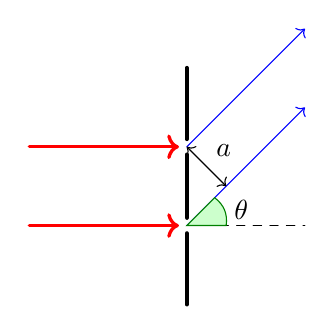
\begin{tikzpicture}
		[scale=1,line cap=round,
		%Styles
		axes/.style=,
		important line/.style={very thick},
		information text/.style={rounded corners,fill=red!10,inner sep=1ex},
		dot/.style={circle,inner sep=1pt,fill,label={#1},name=#1}			
		]
		
		%Colors
		\colorlet{anglecolor}{green!50!black}	%angle arcs/lines
		
		%The graphic
		\draw[black,ultra thick] (0, 1.5) -- (0, .6);
		\draw[black,ultra thick] (0, .4) -- (0, -.4);
		\draw[black,ultra thick] (0, -.6) -- (0, -1.5);
		
		\draw[red,very thick,->] (-2, .5) -- (-.1, .5);
		\draw[red,very thick,->] (-2, -.5) -- (-.1, -.5);
		
		\draw[blue,->] (0, .5) -- (1.5, 2);
		\draw[blue,->] (0, -.5) -- (1.5, 1);
		
		\draw[dashed] (0, -.5) -- (1.5, -.5);
		\coordinate (A) at (0, -.5);
		\coordinate (B) at (1.5, -.5);
		\coordinate (C) at (1.5, 1);
		\coordinate (P) at (0, .5);
		
		\filldraw[fill=green!20,draw=anglecolor] (A) -- ($(A)!5mm!(B)$) to[bend right] node[right,black] {$\theta$} ($(A)!5mm!(C)$) -- cycle;
		
		\draw[<->] (0, .5) -- node[above right] {$a$} ($(A)!(P)!(C)$);
	\end{tikzpicture}
	\end{center}
	
	The only source of phase difference when the two waves meet is the difference in distance traveled, given by $\Delta = a\sin\theta$. The phase difference $\Delta \phi = ka\sin\theta$ then, and the intensity, proportional to the amplitude of the resultant wave squared, is given by
	\begin{equation}
		I \propto 4A^2\cos^2\left( \frac{\pi a \sin\theta}{\lambda} \right)
	\end{equation}
%	\begin{center}
%	\begin{tikzpicture}
%		[scale=3,line cap=round,
%		%Styles
%		axes/.style=,
%		important line/.style={very thick},
%		information text/.style={rounded corners,fill=red!10,inner sep=1ex},
%		dot/.style={circle,inner sep=1pt,fill,label={#1},name=#1}			
%		]
%		
%		%Colors
%		\colorlet{anglecolor}{green!50!black}	%angle arcs/lines
%		
%		%The graphic
%	\end{tikzpicture}
%	\end{center}

%	\begin{figure}[htb]
%		\centering
%		\includegraphics[width=0.8\textwidth]{filename.eps}
%		\caption{Caption.}
%		\label{fig:figure}
%	\end{figure}

%		\def\enotesize{\normalsize}
%		\theendnotes
\end{document}